\documentclass[a4paper,10pt,twoside]{article}

\usepackage[english]{babel}
\usepackage{amssymb}
\usepackage{fancyhdr}
\usepackage{graphicx}
\usepackage[ocgcolorlinks]{hyperref}
\usepackage{todonotes}
\usepackage{caption}
\usepackage{subcaption}

\pagestyle{fancy}
\fancyhead{}
\fancyfoot{}
\fancyhead[RE,LO]{de Kok \& Methenitis}
\fancyhead[RO,LE]{Week 5 \& 6}
\fancyfoot[RE]{\thepage$\quad \square$}
\fancyfoot[LO]{$\square \quad$\thepage}

\title{Report for Week 5 \& 6\\\normalsize Create your own ``Google Similar Images'' system}

\author{Patrick de Kok (5640318) \and Georgios Methenitis (10407537)}

\begin{document}
\maketitle
\thispagestyle{empty}

\section{Implement $k$-NN classifier}
As asked for, the most similar images to the four query images \texttt{goal/15.jpg}, \texttt{bicycle/37.jpg}, \texttt{beach/31.jpg} and \texttt{mountain/37.jpg} are drawn in the report.  The images can be found in Figure~\ref{f:knns}.

\begin{figure}
  \begin{subfigure}{.47\textwidth}
    \centering
    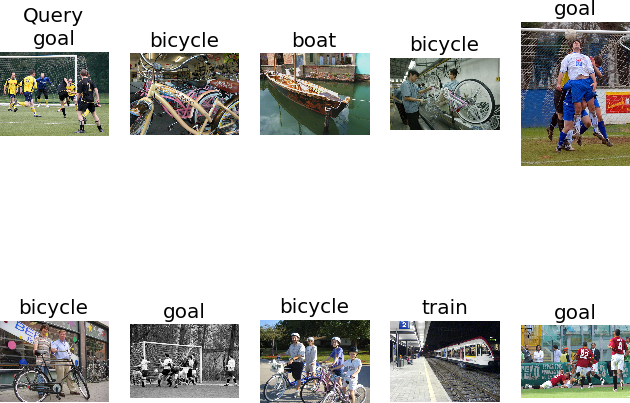
\includegraphics[width=1\textwidth]{knn_goal15}
    \caption{Query image \texttt{goal/15.jpg}.}
  \end{subfigure}
  \hspace*{\fill}
  \begin{subfigure}{.47\textwidth}
    \centering
    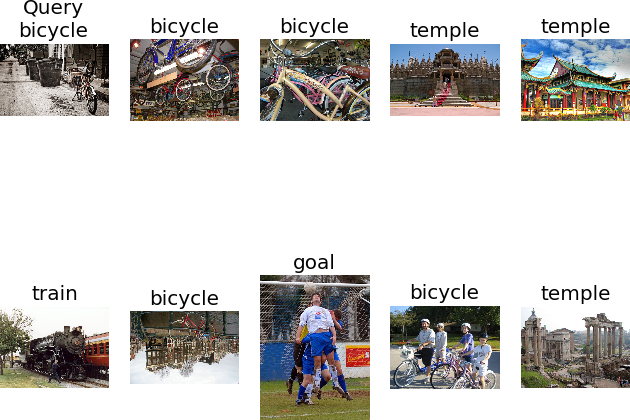
\includegraphics[width=1\textwidth]{knn_bicycle37}
    \caption{Query image \texttt{bicycle/37.jpg}.}
  \end{subfigure}

  \begin{subfigure}{.47\textwidth}
    \centering
    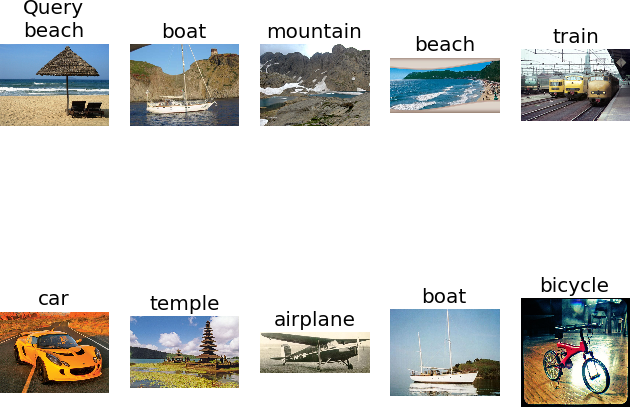
\includegraphics[width=1\textwidth]{knn_beach31}
    \caption{Query image \texttt{beach/31.jpg}.}
  \end{subfigure}
  \hspace*{\fill}
  \begin{subfigure}{.47\textwidth}
    \centering
    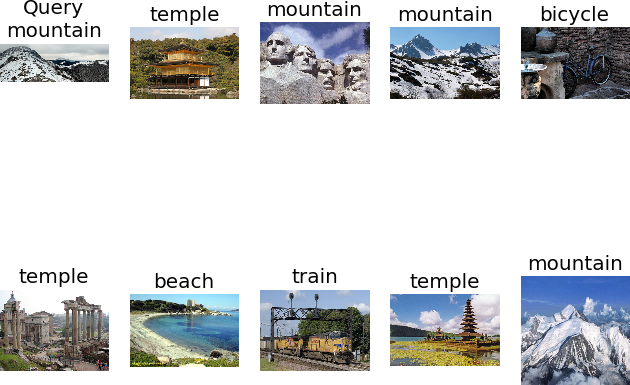
\includegraphics[width=1\textwidth]{knn_mountain37}
    \caption{Query image \texttt{mountain/37.jpg}.}
  \end{subfigure}
  \caption{Query images and their $k=9$ nearest neighbours with labels.}
  \label{f:knns}
\end{figure}

\section{Different $k$-NN strategy}
A possible alternative to this simple voting mechanism will be by weighing each vote based on its rank.  Each vote with rank $r$ will be assigned a weight \[ w_r = \frac{1}{1+r}. \]  Images with a higher rank should be considered as more important than lower ranked images.  The addition of 1 to the rank in the denominator lets the first vote have less relative significance to the second and third votes, such that $w_1 < w_2 + w_3$.

Another weighing mechanism would be based on the global label frequency.  Votes for each label would be weighed by: \[ w_\ell = \frac{1}{\#\ell} \] where $\#\ell$ represents the frequency of label $\ell$ occurring among the training images.  One might want to normalize these weights before they are used, such that \[\bar w_\ell = \frac{w_\ell}{\sum_{\ell \in L} w_\ell}. \] Here, $L$ is the set of all labels.  This ensures that \[\sum_{\ell \in L} w_\ell = 1.\] By weighing votes of very frequent labels less and very infrequent labels more, we tell the system that when a rare (or common) label is suspected to occur in the image this is very (or less) significant than expected.

With training sets of limited size, one is often interested in applying a smoothing method over these weights, such as Good-Turing smoothing.  This will even out the pure chance occurance of very frequent labels and very infrequent labels.  Because this dataset has equal frequencies for all labels, this method is not applicable, and only the first method is implemented.

The accuracy for the original $k$-NN implementation over the four queries is $0.5$, while the alternative implementation has an accuracy of $0.25$.  When inspecting the nearest neighbours of the four queries visually, it becomes clear that the histogram intersection distance is not appropriate for this domain.  The best label is most often not the first returned by $k$-NN.

\section{Implement mean class accuracy}
The accuracy evaluation measure has been implemented, and both $k$-NN label selection mechanisms are evaluated with $k=9$.  The accuracies of both methods per image class and the mean accuracy can be found in Table~\ref{t:classacc}.  Overall both methods have difficulties classifying images correctly.  

\begin{table}
  \centering
  \begin{tabular}{l|rr}
    Class & Original $k$-NN & Alternative $k$-NN \\
    \hline
    Airplane & 0.5 & 0.2 \\
    Beach & 0.1 & 0.1 \\
    Bicycle & 0.8 & 0.7 \\
    Boat & 0.2 & 0.3 \\
    Car & 0.4 & 0.2 \\
    Flower & 0.4 & 0.3 \\
    Goal & 0.1 & 0.2 \\
    Mountain & 0.3 & 0.2 \\
    Temple & 0.3 & 0.3 \\
    Train & 0.0 & 0.1 \\
    \hline
    \emph{Mean accuracy} & 0.31 & 0.26
  \end{tabular}
  \caption{Class accuracy per class and the mean accuracy over the complete test set with the original $k$-NN.}
  \label{t:classacc}
\end{table}

\section{Cross validation of $k$}
The mean class accuracy for each value of $k \in \left\{1, 3, 5, 7, 9, 15\right\}$ is reported in Table~\ref{t:crossacc}.  This has only been computed for the label selection mechanism as meant in the first question.  With $k=9$, you will get the highest mean accuracy.

\begin{table}
  \centering
  \begin{tabular}{l|rrrrrr}
    Label &  $k=1$ &  $k=3$ &  $k=5$ &  $k=7$ &  $k=9$ &  $k=15$ \\
    \hline
    Airplane  & 0.120  & 0.262  & 0.201  & 0.181  & 0.222  & 0.181 \\
       Beach  & 0.312  & 0.348  & 0.332  & 0.257  & 0.173  & 0.201 \\
     Bicycle  & 0.459  & 0.685  & 0.597  & 0.623  & 0.645  & 0.702 \\
        Boat  & 0.348  & 0.363  & 0.363  & 0.458  & 0.423  & 0.423 \\
         Car  & 0.261  & 0.244  & 0.283  & 0.350  & 0.311  & 0.333 \\
      Flower  & 0.486  & 0.399  & 0.418  & 0.381  & 0.401  & 0.374 \\
        Goal  & 0.156  & 0.062  & 0.130  & 0.124  & 0.084  & 0.068 \\
    Mountain  & 0.308  & 0.153  & 0.281  & 0.329  & 0.446  & 0.467 \\
      Temple  & 0.160  & 0.080  & 0.197  & 0.192  & 0.210  & 0.234 \\
       Train  & 0.097  & 0.013  & 0.013  & 0.013  & 0.000  & 0.000 \\
    \hline
  \emph{Mean} & 0.274  & 0.266  & 0.284  & 0.292  & 0.294  & 0.292 \\
  \end{tabular}
  \caption{Class accuracies and mean accuracy for different values of $k$ with threefold cross validation.  As can be concluded from the mean, the classifier performs best with $k=9$.}
  \label{t:crossacc}
\end{table}

\section{Evaluation of 4 possible classifiers}

\section{Use scikit}

\section{Ring data -- linear SVM}

\section{Non-linear transformations}

\section{Transform to polar coordinates}

\section{Non-linear SVM}

\section{Image classification -- linear SVM}

\section{Image classification -- discussing the results}

\section{Image classification -- comparison $k$-NN vs SVM}


%\bibliographystyle{plain}
%\bibliography{thereference}
\end{document}
